\documentclass{beamer}

\mode<presentation>{}

\usetheme{Madrid}

%% preamble
\title{Towards Unification for Dependent Types}
\author[N. Xie, B.C.d.S. Oliveira]
{\textbf{Ningning Xie}, Bruno C. d. S. Oliveira}

\institute[]{The University of Hong Kong}

\date[TFP 2017]{June 2017}


%% custom setting

\usepackage{listings}
\usepackage{fnpct}
\setbeamerfont{footnote}{size=\tiny}

\usepackage{listings}
\lstdefinestyle{fun}{
  aboveskip=0.5\baselineskip,
  belowskip=0.5\baselineskip,
  keepspaces=true,
  mathescape=true,
  columns=fullflexible,
  basicstyle=\fontfamily{cmr}\selectfont\small,
  xleftmargin=10pt,
  keywordstyle=\bfseries,
  identifierstyle=\itshape,
  emphstyle=\fontfamily{cmss}\selectfont,
  commentstyle=\fontfamily{cmtt}\selectfont,
  emph={},
  keywords={where, let, in, case, of, data, newtype, ret, if, then,
    else, defrec, def},
  morecomment=[l]{--},
  literate={
    {->}{{$\to$}}1
    {=>}{{$\To$}}1
    {~}{{$\eq$}}1
    {\\}{{$\lambda$}}1
    {/}{{$\mu$}}1
    {\\~}{{$\lambda_\eq$}}1
    {|->}{{$\mapsto$}}1
    {~>}{{$\leadsto$}}1
    {*}{{$\star$}}1
    {**}{{$\times$}}1
    {++}{{+\kern-1.0ex+\kern1.1ex}}1
    {<}{{$\langle$}}1
    {>}{{$\rangle$}}1
    {|=}{{$\vDash$}}1
    {|-}{{$\vdash$}}1
    {||-}{{$\Vdash$}}1
    {G}{{$\Gamma$}}1
    {G0}{{$\cdot$}}1
    {|>}{{$\vartriangleright$}}1
    {forall}{{$\forall$}}1
    {'}{{$^\prime$}}1
    {_1}{{$_1$}}1
    {_2}{{$_2$}}1
    {^2}{{$^2$}}1
    {@}{{$\bullet$}}1
    {@t}{{$\tau$}}1
    {@s}{{$\sigma$}}1
    {castu2}{{$\fun{cast}_\uparrow^2$}}1
    {castd2}{{$\fun{cast}_\downarrow^2$}}1
    {castuf}{{$\fun{cast}_\uparrow^{\fun{f}}$}}1
    {castup}{{$\fun{cast}_\uparrow$}}1
    {castdn}{{$\fun{cast}_\downarrow$}}1
  }
}
\lstset{style=fun}
\newcommand{\lst}[1]{\text{\lstinline$#1$}}

% Table
\usepackage{multirow}
\usepackage{tabularx}
\newcolumntype{Y}{>{\centering\arraybackslash}X}
\newcolumntype{Z}{>{\raggedleft\arraybackslash}X}

% Infer rules
\usepackage{mathpartir}
\newcommand{\rname}[1]{{\,\text{\scriptsize \textsc{#1}}}}
\newcommand{\rul}[1]{\textsc{#1}}

% Extra symbols
\usepackage{stmaryrd}

% Macros for math typesetting

%% Names
% \newcommand{\name}{{\bf $\lambda_{\mu}^{\eq}$}\xspace}

%% Symbols
\newcommand{\syndef}{$::=$}
\newcommand{\synor}{$\mid$}
\newcommand{\syneq}{$\triangleq$}
\newcommand{\header}[1]{\multicolumn{1}{l}{$\boxed{#1}$}}
\newcommand{\headercap}[2]{\multicolumn{1}{l}{$\boxed{#1}$\quad{#2}}}
\newcommand{\headercapm}[2]{\vspace{1pt}\raggedright \framebox{\mbox{$#1$}} \quad
  #2}
\newcommand{\headercapt}[2]{\framebox{\mbox{$#1$}} \quad #2}

%% Arrows
\newcommand{\To}{\Rightarrow}
\newcommand{\Chk}{\Downarrow}
\newcommand{\Inf}{\Uparrow}
\newcommand{\Inst}{{inst}}
\newcommand{\Gen}{{gen}}
\newcommand{\redto}{\hookrightarrow}
\newcommand{\redton}{\hookrightarrow^*}
\newcommand{\eq}{\sim}
\newcommand{\lt}{\sqsubseteq}
\newcommand{\sugar}{\triangleq}
%\newcommand{\trto}[1]{\hl{\rightsquigarrow #1}}
\newcommand{\trto}[1]{}
\newcommand{\opt}[1]{}
\newcommand{\trtop}{\rightsquigarrow}

%% Styles
\newcommand{\kw}[1]{\operatorname{\mathbf{#1}}}
\newcommand{\var}{\mathit}
\newcommand{\fun}{\mathsf}

%% Constructs
\newcommand{\bind}[3]{#1 #2:#3.~}
\newcommand{\blam}{\bind \lambda}
\newcommand{\bmu}{\bind \mu}
\newcommand{\barr}[2]{(#1:#2) \to}

\newcommand{\bindv}[4][]{#2\,\overline{#3:#4}^{#1}.~}
\newcommand{\blamv}[3][]{\bindv[#1] \lambda {#2} {#3}}
\newcommand{\bmuv}[3][]{\bindv[#1] \mu {#2} {#3}}
\newcommand{\barrv}[3][]{\overline{#2:#3}^{#1} \to}

\newcommand{\eqlam}[2]{\lambda_{\eq}({#1} \eq {#2}).~}
\newcommand{\eqty}[2]{({#1} \eq {#2})\Rightarrow}
\newcommand{\eqapp}[2][]{\langle {#2} \rangle^{#1}}
\newcommand{\eqlamv}[3][]{\lambda_{\eq}\overline{{#2} \eq {#3}}^{#1}.~}
\newcommand{\eqtyv}[3][]{\overline{({#2} \eq {#3})}^{#1}\Rightarrow}

\newcommand{\bpi}{\bind \Pi}
\newcommand{\bpiv}[3][]{\bindv[#1] \Pi {#2} {#3}}

\newcommand{\fold}{\fun{fold}}
\newcommand{\unfold}{\fun{unfold}}

\newcommand{\castupz}{\fun{cast}_\uparrow}
\newcommand{\castup}[2][]{\fun{cast}_\uparrow^{#1}~[#2]~}
\newcommand{\castdnz}{\fun{cast}_\downarrow}
\newcommand{\castdn}[1][]{\fun{cast}_\downarrow^{#1}~}
\newcommand{\castdnt}[2][]{\fun{cast}_\downarrow^{#1}~[#2]~}
\newcommand{\subst}[2]{[#1 \mapsto #2]}
\newcommand{\Subst}[2]{[#1 \Mapsto #2]}
\newcommand{\substv}[3][]{\overline{[#2 \mapsto #3]}^{#1}}
\newcommand{\cast}[2][]{\fun{cast}^{#1}~[#2]~}

\newcommand{\triv}{\_}
\newcommand{\trivtm}{\bullet}
\newcommand{\er}[1]{|{#1}|}
\newcommand{\erf}[1]{\|{#1}\|}
\newcommand{\erlam}[1]{\lambda {#1}.~}
\newcommand{\ermu}[1]{\mu {#1}.~}
\newcommand{\ercastup}{\castupz~}
\newcommand{\ereqlam}{\lambda_\eq.~}

\newcommand{\genvar}{\widehat}
\newcommand{\genA}{\genvar{\alpha}}
\newcommand{\genB}{\genvar{\beta}}
\newcommand{\varA}{\alpha}
\newcommand{\varB}{\beta}

%% Context
\newcommand{\dctx}{\Psi}
\newcommand{\tctx}{\Gamma}
\newcommand{\ctxinit}{\varnothing}
\newcommand{\ctxl}{\Theta}
\newcommand{\ctxr}{\Delta}
\newcommand{\cctx}{\Omega}
\newcommand{\byuni}{\vdash}
\newcommand{\byinf}{\vdash_\Inf}
\newcommand{\bychk}{\vdash_\Chk}
\newcommand{\byapp}{\vdash_\bullet}
\newcommand{\byall}{\vdash_\delta}
\newcommand{\bytar}{\vdash}
\newcommand{\byinst}{\vdash_\Inst}
\newcommand{\bygen}{\vdash_\Gen}
\newcommand{\bycg}{\vdash}
\newcommand{\bywf}{\vdash}
\newcommand{\bywt}{\vDash}
\newcommand{\toctx}{\dashv \ctxl}
\newcommand{\toctxo}{\dashv \tctx}
\newcommand{\toctxr}{\dashv \ctxr}
\newcommand{\dpreinf}[1][]{\dctx {#1} \byinf}
\newcommand{\dprechk}[1][]{\dctx {#1} \bychk}
\newcommand{\dpreall}[1][]{\dctx {#1} \byall}
\newcommand{\dpreapp}[1][]{\dctx {#1} \byapp}
\newcommand{\dpreuni}[1][]{\dctx {#1} \byuni}
\newcommand{\dpretar}[1][]{\dtctx {#1} \bytar}
\newcommand{\dpreinst}[1][]{\dctx {#1} \byinst}
\newcommand{\dpregen}[1][]{\dctx {#1} \bygen}
\newcommand{\dprecg}[1][]{\dctx {#1} \bycg}
\newcommand{\dprewf}[1][]{\dctx {#1} \bywf}
\newcommand{\dprewt}[1][]{\dctx {#1} \bywt}
\newcommand{\tpreinf}[1][]{\tctx {#1} \byinf}
\newcommand{\tprechk}[1][]{\tctx {#1} \bychk}
\newcommand{\tpreall}[1][]{\tctx {#1} \byall}
\newcommand{\tpreapp}[1][]{\tctx {#1} \byapp}
\newcommand{\tpreuni}[1][]{\tctx {#1} \byuni}
\newcommand{\tpretar}[1][]{\ttctx {#1} \bytar}
\newcommand{\tpreinst}[1][]{\tctx {#1} \byinst}
\newcommand{\tpregen}[1][]{\tctx {#1} \bygen}
\newcommand{\tprecg}[1][]{\tctx {#1} \bycg}
\newcommand{\tprewf}[1][]{\tctx {#1} \bywf}
\newcommand{\tprewt}[1][]{\tctx {#1} \bywt}
\newcommand{\wc}{\ \var{ctx}\ }
\newcommand{\exto}{\longrightarrow}
\newcommand{\cgto}{\longmapsto}

% Primitives
\newcommand{\Int}{\var{Int}}
\newcommand{\String}{\var{String}}

\newcommand{\overbar}[1]{\mkern 1.5mu\overline{\mkern-1.5mu#1\mkern-1.5mu}\mkern 1.5mu}

%%% Local Variables:
%%% mode: latex
%%% TeX-master: "main"
%%% End:



%% begin
\begin{document}

% Setup spaces between column
\setlength{\tabcolsep}{2pt}

%Complete Contexts &
%$\cctx$ & \syndef & $\ctxinit \mid \ctx,x \mid \ctx,x:\tau \mid \ctx,x:\tau=\tau_2$ \\
%&& \synor & $\ctx,\genA=\tau$ \\

% ------------------------------------------------------------------------
% TYPING RULES
% ------------------------------------------------------------------------

\newcommand*{\TAx}{\inferrule{ }{\preinf \star:\star \toctxo}\rname{T-Ax}}
\newcommand*{\TVar}{\inferrule{x:\tau \in \ctx}{\preinf x:\tau \toctxo
  }\rname{T-Var}}
\newcommand*{\TLetVar}{\inferrule{x:\sigma = \tau \in \ctx \\ \preinst \sigma \lt \tau_2 \toctx}{\preinf x:\tau_2 \toctx
  }\rname{T-LetVar}}
\newcommand*{\TSub}{\inferrule{\preinf e : \tau_1 \toctx_1 \\ \ctxl_1 \byuni [\ctxl_1]\tau_1
    \lt [\ctxl_1]\tau_2 \toctx}{\prechk e:\tau_2 \toctx }\rname{T-Sub}}
\newcommand*{\TAnn}{\inferrule{\prechk \tau:\star \toctx_1 \\
    \ctxl_1 \bychk e:\tau \toctx }{\preinf (e:\tau):\tau \toctx
  }\rname{T-Ann}}
\newcommand*{\TLamInf}{\inferrule{\preinf[,\genA,x:\genA]
    e:\tau_2 \toctx, x:\genA, \ctxr }{\preinf \erlam x e : (\bpi x \genA
    [\ctxr]\tau_2) \toctx, UV(\ctxr) }\rname{T-Lam$\Inf$}}
\newcommand*{\TLamChk}{\inferrule{\prechk[,x:\tau_1]
    e:\tau_2 \toctx,x:\tau_1,\ctxr \\
    \opt{\prechk {\tau_1 : \star \toctx_1 }}
    }{\prechk \erlam x e : \bpi x {\tau_1}
    \tau_2 \toctx }\rname{T-Lam$\Chk$}}
\newcommand*{\TLamAnnInf}{\inferrule{\prechk \tau_1 : \star \toctx_1\\
    \ctxl_1,x:\tau_1 \byinf
    e:\tau_2 \toctx, x:\tau_1, \ctxr }{\preinf \blam x {\tau_1} e : (\bpi x {\tau_1}
    [\ctxr]\tau_2) \toctx, UV(\ctxr) }\rname{T-LamAnn$\Inf$}}
\newcommand*{\TLamAnnChk}{\inferrule{\prechk \tau_1 : \star \toctx_1\\
    \ctxl_1 \byuni [\ctxl_1] \tau_1 \lt [\ctxl_1] \tau_3 \toctx_2 \\
    \ctxl_2,x:\tau_1 \bychk
    e:\tau_2 \toctx, x:\tau_1, \ctxr }
    {\prechk \blam x {\tau_1} e : (\bpi x {\tau_3} \tau_2) \toctx }\rname{T-LamAnn$\Chk$}}
\newcommand*{\TApp}{\inferrule{
    \preinf e_1 : \tau_1 \toctx_1 \\
    \ctxl_1 \byapp [\ctxl_1]\tau_1~e_2 : \tau_2 \toctx \\
}{\preinf e_1~e_2:\tau_2 \toctx}\rname{T-App}}
\newcommand*{\TAppPi}{\inferrule{
    \preinf e_1 : \bpi x {\tau_1} \tau_2 \toctx_1 \\
    \ctxl_1 \bychk e_2 : [\ctxl_1]\tau_1 \toctx \\
}{\preinf e_1~e_2:\tau_2 \subst x
    {e_2} \toctx}\rname{T-AppPi}}
\newcommand*{\TAppVar}{\inferrule{
    \preinf e_1 : \genA \toctx_1[\genA] \\
    \ctxl_1[\genA_1,\genA_2,\genA=\bpi x {\genA_1} \genA_2] \bychk e_2 : \genA_1 \toctx \\
}{\preinf e_1~e_2:\genA_2 \toctx}\rname{T-AppVar}}
\newcommand*{\TPi}{\inferrule{\prechk \tau_1 : \star \toctx_1 \\
\ctxl_1,x:\tau_1 \bychk \tau_2 : \star \toctx,x:\tau_1,\ctxr}{\preinf \bpi x {\tau_1} {\tau_2} :
    \star \toctx }\rname{T-Pi}}
\newcommand*{\TLet}{\inferrule{\preinf e_1 : \tau_1 \toctx_1  \\
\ctxl_1 \bygen {\tau_1} \lt \sigma \\
\ctxl_1, x:\sigma = e_1 \byall e_2 : \tau_2 \toctx, x:\sigma = e_1, \ctxr }{\preall \kw{let} x=e_1
\kw{in} e_2 : [x:\sigma=e_1, \ctxr]\tau_2 \toctx, UV(\ctxr) }\rname{T-Let}}
\newcommand*{\TCastUp}{\inferrule{[\ctx]\tau_2
    \redto \tau_1 \\
    \prechk e : \tau_1 \toctx \\
    \opt{\prechk \tau_1 : \star \toctx_1}
    }
  {\prechk \ercastup e : \tau_2 \toctx
    }\rname{T-CastUp}}
\newcommand*{\TCastDn}{\inferrule{\preinf e : \tau_1 \toctx \\
    [\ctxl]\tau_1 \redto \tau_2}{\preinf \castdn e : \tau_2
    \toctx }\rname{T-CastDn}}

% DECLARATIVE

\newcommand*{\DAx}{\inferrule{ }{\preinf \star:\star \trto \star}\rname{D-Ax}}
\newcommand*{\DVar}{\inferrule{x:\tau \in \ctx}{\preinf x:\tau
  \trto x}\rname{D-Var}}
\newcommand*{\DLetVar}{\inferrule{x:\sigma = \tau \in \ctx \\ \preinst \sigma \lt \tau_2 \trto f}{\preinf x:\tau_2
  \trto {f~x}}\rname{D-LetVar}}
\newcommand*{\DSub}{\inferrule{\preinf e : \tau \trto{t}}
  {\prechk e:\tau  \trto{t}}\rname{D-Sub}}
\newcommand*{\DAnn}{\inferrule{\prechk \tau:\star \\
    \ctx \bychk e:\tau  \trto t}{\preinf (e:\tau):\tau
  \trto t}\rname{D-Ann}}
\newcommand*{\DLamInf}{\inferrule{ \prechk \tau_1 : \star \trto {t_1} \\ \preinf[,x:\tau_1]
    e:\tau_2 \trto {t_2}}{\preinf \erlam x e : (\bpi x {\tau_1} {\tau_2})
    \trto {\blam x {t_1} {t_2}}}\rname{D-Lam$\Inf$}}
\newcommand*{\DLamChk}{\inferrule{\prechk[,x:\tau_1]
    e:\tau_2 \trto {t_2} \\
    \opt{\prechk {\tau_1 : \star  \trto {t_1}}}
    }{\prechk \erlam x e : (\bpi x {\tau_1} \tau_2)  \trto {\blam x {t_1} t_2}}\rname{D-Lam$\Chk$}}
\newcommand*{\DLamAnnInf}{\inferrule{\prechk \tau_1 : \star
    \trto {t_1} \\
    \ctx,x:\tau_1 \byinf
    e:\tau_2\trto {t_2}}{\preinf \blam x {\tau_1} e : (\bpi x {\tau_1}
    \tau_2) \trto {\blam x {t_1} t_2}}\rname{D-LamAnn$\Inf$}}
\newcommand*{\DLamAnnChk}{\inferrule{
    \ctx,x:\tau_1 \bychk
    e:\tau_2\trto {t_2}}{\prechk \blam x {\tau_1} e : (\bpi x {\tau_1}
    \tau_2) \trto {\blam x {t_1} t_2}}\rname{D-LamAnn$\Chk$}}
\newcommand*{\DApp}{\inferrule{
    \preinf e_1 : \bpi  x {\tau_1} {\tau_2} \trto {t_1} \\
    \prechk e_2 : \tau_1 \trto {t_2}
}{\preinf e_1~e_2:\tau_2 \subst x {e_2}  \trto {t_1~t_2}}\rname{D-App}}
\newcommand*{\DPi}{\inferrule{\prechk \tau_1 : \star \trto {t_1} \\
\ctx,x:\tau_1 \bychk \tau_2 : \star \trto {t_2}}{\preinf \bpi x {\tau_1} {\tau_2} :
    \star \trto {\bpi x {t_1} t_2}}\rname{D-Pi}}
\newcommand*{\DLet}{\inferrule{\pregen e_1 : \sigma \trto {t_1} \\
\ctx, x:\sigma = e_1 \byall e_2 : \tau_2 \trto {t_2}}{\preall \kw{let} x=e_1
\kw{in} e_2 : \tau_2 \subst x {e_1} \trto {\kw{let} x = t_1 \kw{in} t_2}}\rname{D-Let}}
\newcommand*{\DCastUp}{\inferrule{\tau_2 \redto \tau_1 \\
    \prechk e : \tau_1 \trto {t_2} \\
    \opt{\prechk \tau_1 : \star \trto {t_1}}
    }
  {\prechk \ercastup e : \tau_2
    \trto {\castup {t_1} t_2}}\rname{D-CastUp}}
\newcommand*{\DCastDn}{\inferrule{\preinf e : \tau_1\trto t \\
    \tau_1 \redto \tau_2}{\preinf \castdn e : \tau_2
    \trto {\castdn t}}\rname{D-CastDn}}
\newcommand*{\DConv}{\inferrule{\preinf e_1 : \tau_1 \trto t \\ [\ctx]\tau_1 = [\ctx]\tau_2}
    {\preinf e_1 : \tau_2 \trto t}\rname{D-Conv}}

\newcommand*{\DPoly}{\inferrule{\prechk[x:\star] \sigma : \star \trto {t}}
{\preinf \forall x:\star. \sigma : \star \trto {\bpi x \star t}}\rname{D-Poly}}

\newcommand*{\DInstantiation}{\inferrule{\prechk \overbar{\tau} : \star \trto {\overbar t} \\
\sigma = \forall{\overbar{x:\star}}. \tau_1 \\
\opt{\prechk \sigma : \star \trto{t_1}}
}
{\preinst \sigma \lt \tau_1[\overbar{x} \mapsto \overbar{\tau}] \trto {\blam x {t_1} x ~ \overbar{t}}
} \rname{D-Inst}}

\newcommand*{\DGeneralization}{\inferrule{ \preinf[, \overbar{x:\star}] e : \tau \trto {t_1}
\\  \overbar x \notin FV(e)}
{\pregen e : \forall \overbar{x:\star}. \tau
\trto {(\blam {x_1} \star {\blam {x_2} \star {... \blam {x_n} \star {t_1}}})}} \rname{D-Gen}}

% ------------------------------------------------------------------------
% UNIFICATION RULES
% ------------------------------------------------------------------------

\newcommand*{\UVar}{\inferrule{ }{\preuni[{[x]}] x \lt x \toctxo[x]}\rname{U-Var}}
\newcommand*{\UEVarId}{\inferrule{ }{\preuni[{[\genA]}] \genA \lt \genA \toctxo[\genA]}\rname{U-EVarId}}
\newcommand*{\UEVarTy}{\inferrule{\genA \not \in \fun{FV}(\tau_1) \\ \ctx[\genA] \bycg \tau_1 \cgto \tau_2 \toctx_1, \genA, \ctxl_2 \\ \ctxl_1 \bywt \tau_2}
{\ctx[\genA] \byuni \genA \lt \tau_1 \toctx_1, \genA=\tau_2, \ctxl_2}\rname{U-EvarTy}}
\newcommand*{\UTyEVar}{\inferrule{\genA \not \in \fun{FV}(\tau_1) \\ \ctx[\genA] \bycg \tau_1 \cgto \tau_2 \toctx_1, \genA, \ctxl_2 \\ \ctxl_1 \bywt \tau_2}
{\ctx[\genA] \byuni \tau_1 \lt \genA \toctx_1, \genA=\tau_2, \ctxl_2}\rname{U-TyEVar}}
\newcommand*{\UStar}{\inferrule{ }{\preuni \star \lt \star \toctxo}\rname{U-Star}}
\newcommand*{\UApp}{\inferrule{\preuni \tau_2 \lt \tau_2' \toctx_1 \\
    \ctxl_1 \byuni [\ctxl_1]\tau_1 \lt [\ctxl_1]\tau_1'
    \toctx}{\preuni \tau_1~\tau_2 \lt \tau_1'~\tau_2'
    \toctx}\rname{U-App}}
\newcommand*{\ULam}{\inferrule{\preuni[,x] \tau \lt \tau'
    \toctx,x,\ctxr}{\preuni \erlam x \tau \lt \erlam x \tau' \toctx}\rname{U-Lam}}
\newcommand*{\ULamAnn}{\inferrule{\preuni \tau_1 \lt \tau_3 \toctx_1 \\
    \ctxl_1, x:\tau_1 \byuni [\ctxl_1]\tau_2 \lt [\ctxl_1]\tau_4
    \toctx,x:\tau_1,\ctxr}{\preuni \blam x {\tau_1} \tau_2 \lt \blam x
    {\tau_3} \tau_4 \toctx}\rname{U-LamAnn}}
\newcommand*{\UPi}{\inferrule{\preuni \tau_1' \lt \tau_1 \toctx_1
    \\ \ctxl_1,x:\tau_1 \byuni [\ctxl_1]\tau_2 \lt [\ctxl_1]\tau_2'
    \toctx,x:\tau_1,\ctxr}{\preuni \bpi x {\tau_1} \tau_2 \lt \bpi x
    {\tau_1'} \tau_2' \toctx}\rname{U-Pi}}
\newcommand*{\ULet}{\inferrule{\preuni \tau_1 \lt \tau_1' \toctx_1
    \\ \ctxl_1, x \byuni {[\ctxl_1]}\tau_2 \lt [\ctxl_1]\tau_2'
    \toctx, x, \ctxr}{\preuni \kw{let} x ={\tau_1} \kw{in} \tau_2 \lt \kw{let} x=
    {\tau_1'} \kw{in} \tau_2' \toctx}\rname{U-Let}}
\newcommand*{\UCastUp}{\inferrule{\preuni \tau \lt \tau'
    \toctx}{\preuni \ercastup \tau \lt \ercastup \tau' \toctx}\rname{U-CastUp}}
\newcommand*{\UCastDn}{\inferrule{\preuni \tau \lt \tau'
    \toctx}{\preuni \castdn \tau \lt \castdn \tau' \toctx}\rname{U-CastDn}}
\newcommand*{\UAnn}{\inferrule{\preuni \tau \lt \tau' \toctx_1 \\
    \ctxl_1 \byuni [\ctxl_1]e \lt [\ctxl_1]e'
    \toctx}{\preuni e:\tau \lt e':\tau'
    \toctx}\rname{U-Ann}}

% ------------------------------------------------------------------------
% APPLICATION RULES
% ------------------------------------------------------------------------

\newcommand*{\APi}{\inferrule{\prechk e:\tau_1 \toctx \trto t}{\preapp (\bpi x
    {\tau_1} \tau_2)~e : \tau_2[x \mapsto e] \toctx \trto t}\rname{A-Pi}}
\newcommand*{\AEVar}{\inferrule{\prechk[{[\genA_2,\genA_1,\genA=\bpi x
    {\genA_1} \genA_2]}] e : \genA_1 \toctx \trto t}{\preapp[{[\genA]}]
  \genA~e : \genA_2 \toctx \trto t}\rname{A-EVar}}

% ------------------------------------------------------------------------
% TARGET TYPING RULES
% ------------------------------------------------------------------------

\newcommand*{\EAx}{\inferrule{ }{\pretar \star:\star }\rname{E-Ax}}
\newcommand*{\EVar}{\inferrule{x:s \in \tctx}{\pretar x:s}\rname{E-Var}}
\newcommand*{\EApp}{\inferrule{\pretar t_1:\bpi x {s_1} {s_2} \\ \pretar
    t_2:s_1}{\pretar t_1~t_2:s_2 \subst
  x {t_2}}\rname{E-App}}
\newcommand*{\ELam}{\inferrule{\pretar t_1:\star \\ \pretar[,x:t_1] t_2:s_1
    }{\pretar \blam
    x {t_1} t_2 : \bpi x {t_1} {s_1}}\rname{E-Lam}}
\newcommand*{\EPi}{\inferrule{\pretar t_1:\star \\ \pretar[,x:t_1] t_2:\star }{\pretar \bpi x {t_1} t_2 :
    \star}\rname{E-Pi}}
\newcommand*{\ECastUp}{\inferrule{\pretar t_1 : \star \\ \pretar t_2: s_1 \\ t_1 \redto s_1 }{\pretar \castup {t_1} {t_2} :t_1}\rname{E-CastUp}}
\newcommand*{\ECastDown}{\inferrule{\pretar t_1 : s_1 \\ s_1 \redto s_2 }{\pretar \castdn t_1 :s_2}\rname{E-CastDown}}
\newcommand*{\ELet}{\inferrule{\pretar t_1 : s_1 \\ \pretar[,x:s_1=t_1] t_2:s_2}{\pretar \kw{let} x = t_1 \kw{in} t_2: s_2}\rname{E-Let}}
\newcommand*{\EConv}{\inferrule{\pretar t_1 : s_1 \\ [\tctx]s_1 = [\tctx]s_2}{\pretar t_1 : s_2}\rname{E-Conv}}

% ------------------------------------------------------------------------
% POLYMORPHISM
% ------------------------------------------------------------------------

\newcommand*{\Instantiation}{\inferrule{\sigma = \forall{\overbar{x:\star}}. \tau}{\preinst \sigma \lt \tau[\overbar{x} \mapsto \overbar{\genA}] \toctx, \overbar{\genA}} \rname{Inst}}

\newcommand*{\Generalization}{\inferrule{\tau_2 = [\ctx]\tau \\ \overbar{\genA} = FV(\tau_2) - FV(\ctx)}{\pregen \tau \lt \forall \overbar{x:\star}. \tau_2[\overbar{\genA} \mapsto \overbar{x}]} \rname{Gen}}

% ------------------------------------------------------------------------
% UNIFY TVAR
% ------------------------------------------------------------------------

\newcommand*{\IVar}{\inferrule{ }{\ctx \bycg x \cgto x \toctxo}\rname{I-Var}}
\newcommand*{\IStar}{\inferrule{ }{\ctx \bycg \star \cgto \star \toctxo}\rname{I-Star}}
\newcommand*{\IEVarA}{\inferrule{ }{\ctx[\genB][\genA] \bycg \genB \cgto \genB \toctxo[\genB][\genA]}\rname{I-EVar1}}
\newcommand*{\IEVarB}{\inferrule{ }{\ctx[\genA][\genB] \bycg \genB \cgto \genA_1 \toctxo[\genA_1, \genA][\genB=\genA_1]}\rname{I-EVar2}}
\newcommand*{\IOthers}{\inferrule{\ctx \bycg \tau_0 \cgto \tau_0' \toctx_1 \\ \ctxl_i \bycg [\ctxl_i]\tau_i \cgto \tau_i' \toctx_{i+1}}{\ctx \bycg T\ \overbar{\tau_n} \cgto T\ \overbar{\tau_n'}}\rname{I-Other}}

% ------------------------------------------------------------------------
% WELL FORM
% ------------------------------------------------------------------------

\newcommand*{\WFPoly}{\inferrule{ \prewt[,x:\star] \sigma}{ \prewt \forall x: \star. \sigma}\rname{WF-Poly}}
\newcommand*{\WFOther}{\inferrule{ \prechk \tau : \star}{ \prewt \tau}\rname{WF-Other}}

\newcommand*{\TWFEVar}{\inferrule{\genA \in \ctx }{\prewt \genA}\rname{WF-EVar}}
\newcommand*{\TWFPi}{\inferrule{\prewt \tau_1 \\ \prewt \tau_2 }{\prewt \bpi x {\tau_1} {\tau_2}}\rname{WF-Pi}}
\newcommand*{\TWFPoly}{\WFPoly}
\newcommand*{\TWFOther}{\inferrule{ \prechk \tau : \star \toctx}{ \prewt \tau}\rname{WF-Other}}

\newcommand*{\WCEmpty}{\inferrule{ }{\ctxinit \wc}\rname{WC-Empty}}
\newcommand*{\WCVar}{\inferrule{\ctx \wc \\ x \notin dom(\ctx)}{\ctx, x \wc}\rname{WC-Var}}
\newcommand*{\WCTypedVar}{\inferrule{\ctx \wc \\ x \notin dom(\ctx) \\ \ctx \bywt \tau}{\ctx, x: \tau \wc}\rname{WC-TypedVar}}
\newcommand*{\WCLetVar}{\inferrule{\ctx \wc \\ x \notin dom(\ctx) \\ \ctx \bywt \sigma \\ \sigma = \forall {\overbar {y:\star}}.\tau \\ \prechk[,\overbar{y:\star}] e:\tau}
{\ctx, x:\sigma = e}\rname{WC-LetVar}}

\newcommand*{\TWCEmpty}{\WCEmpty}
\newcommand*{\TWCVar}{\WCVar}
\newcommand*{\TWCTypedVar}{\WCTypedVar}
\newcommand*{\TWCLetVar}{\inferrule{\ctx \wc \\ x \notin dom(\ctx) \\ \ctx \bywt \sigma \\ \sigma = \forall {\overbar {y:\star}}.\tau \\ \prechk[,\overbar{y:\star}] e:\tau\toctx}
{\ctx, x:\sigma = e}\rname{WC-LetVar}}
\newcommand*{\TWCEVar}{\inferrule{\ctx \wc \\ \genA \notin dom(\ctx)}{\ctx, \genA \wc}\rname{WC-EVar}}
\newcommand*{\TWCSolvedEVar}{\inferrule{\ctx \wc \\ \genA \notin dom(\ctx) \\ \ctx \bywt \tau}{\ctx, \genA = \tau \wc}\rname{WC-SolvedEVar}}

% ------------------------------------------------------------------------
% TRANSLATION CONTEXT
% ------------------------------------------------------------------------

\newcommand*{\TCEmpty}{\inferrule{ } {\ctxinit \trtop \ctxinit}\rname{TC-Empty}}
\newcommand*{\TCTypedVar}{\inferrule{\ctx \trtop \tctx \\ \prechk \tau : \star \trtop t} {\ctx, x:\tau \trtop \tctx, x:t}\rname{TC-TypedVar}}
\newcommand*{\TCLetVar}{\inferrule{\ctx \trtop \tctx \\ \prechk \sigma : \star \trtop t_1 \\ \pregen \tau : \sigma \trtop t_2
} {\ctx, x:\sigma = \tau \trtop \tctx, x:t_1 = t_2}\rname{TC-LetVar}}

% ------------------------------------------------------------------------
% CONTEXT EXTENSION
% ------------------------------------------------------------------------

\newcommand*{\CEEmtpy}{\inferrule{  }{\ctxinit \exto \ctxinit}\rname{CE-Empty}}
\newcommand*{\CEVar}{\inferrule{\ctx \exto \ctxr}{\ctx, x \exto \ctxr, x}\rname{CE-Var}}
\newcommand*{\CETypedVar}{\inferrule{\ctx \exto \ctxr \\ [\ctxr]\tau_1 = [\ctxr]\tau_2}{\ctx, x:\tau_1 \exto \ctxr, x:\tau_2}\rname{CE-TypedVar}}
\newcommand*{\CELetVar}{\inferrule{\ctx \exto \ctxr \\ [\ctxr]\tau_1 = [\ctxr]\tau_3 \\ [\ctxr]\tau_2 = [\ctxr]\tau_4}{\ctx, x:\tau_1=\tau_2 \exto \ctxr, x:\tau_3 = \tau_4}\rname{CE-LetVar}}
\newcommand*{\CEEVar}{\inferrule{ }{\ctx, \genA \exto \ctxr, \genA}\rname{CE-EVar}}
\newcommand*{\CESolvedEVar}{\inferrule{\ctx \exto \ctxr \\ [\ctxr]\tau_1 = [\ctxr]\tau_2}{\ctx, \genA = \tau_1 \exto \ctxr, \genA = \tau_2}\rname{CE-SolvedEVar}}
\newcommand*{\CESolve}{\inferrule{\ctx \exto \ctxr \\ \prechk \tau : \star}{\ctx, \genA \exto \ctxr, \genA = \tau}\rname{CE-Solve}}
\newcommand*{\CEAdd}{\inferrule{\ctx \exto \ctxr}{\ctx, \genA \exto \ctxr, \genA}\rname{CE-Add}}
\newcommand*{\CEAddSolved}{\inferrule{\ctx \exto \ctxr \\ \prechk \tau : \star}{\ctx \exto \ctxr, \genA:\tau}\rname{CE-AddSolved}}

% ------------------------------------------------------------------------
% REFERENCE OF ORIGINAL SYSTEM
% ------------------------------------------------------------------------

\newcommand*{\OLamInf}{\inferrule{\prechk[,\genA,\genB,x:\genA]
    e:\genB \toctx, x:\genA, \ctxr}{\preinf \erlam x e : (\bpi x \genA
    \genB) \toctx}\rname{$\rightarrow$ I $\Rightarrow$}}

\newcommand*{\OInstLArr}{\inferrule{\preuni[{[\genA_2, \genA_1, \genA = \genA_1 \to \genA_2]}] \genA_1 \lt A_1 \toctx_1 \\
    \ctxl_1 \byuni [\ctxl_1]A_2 \lt \genA_2 \toctx} {\preuni[{[\genA]}] \genA \lt A_1 \to A_2 \toctx}\rname{InstLArr}}

\newcommand*{\OInstLSolve}{\inferrule{\ctx \bywt \tau}{\ctx, \genA, \ctx' \byuni \genA \lt \tau \toctxo, \genA = \tau, \ctx'}\rname{InstLSolve}}

\newcommand*{\OInstLReach}{\inferrule{ }{\preuni[{[\genA][\genB]}] \genA \lt \genB \toctxo[\genA][\genB=\genA]}\rname{InstLReach}}

% ------------------------------------------------------------------------
% OPERATIONAL SEMANTICS
% ------------------------------------------------------------------------

\newcommand*{\SBetaA}{\inferrule{ }{(\blam x \tau {e_1}) e_2 \redto e_1 \subst x {e_2} }\rname{S-Beta1}}
\newcommand*{\SBetaB}{\inferrule{ }{(\erlam x {e_1}) e_2 \redto e_1 \subst x {e_2}}\rname{S-Beta2}}
\newcommand*{\SApp}{\inferrule{ e_1 \redto e_1' }{e_1~e_2 \redto e_1'~e_2}\rname{S-App}}
\newcommand*{\SCastDownUp}{\inferrule{  }{\castdn (\ercastup e) \redto e}\rname{S-CastDownUp}}
\newcommand*{\SCastDown}{\inferrule{e \redto e'}{\castdn e \redto \castdn e'}\rname{S-CastDown}}
\newcommand*{\SLet}{\inferrule{ }{\kw{let} x = e_1 \kw{in} e_2 \redto e_2 \subst x {e_1}}\rname{S-Let}}
\newcommand*{\SAnn}{\inferrule{e \redto e'}{ e:\tau \redto e':\tau}\rname{S-Ann}}

% ------------------------------------------------------------------------
% EXAMPLES
% ------------------------------------------------------------------------

\newcommand*{\ExUni}{\inferrule{\genA \notin FV(\bpi x \genB x) \quad
                                       \inferrule{\inferrule{ }
                                                            {\ctx,\genA,\genB,\ctxr \bycg \genB \cgto \genA_1 \toctx}\rname{I-Evar2}
                                                  \quad
                                                  \inferrule{ }
                                                            {\ctxl \bycg x \cgto x \toctx}\rname{I-Var}}
                                                 {\ctx,\genA,\genB,\ctxr \bycg \bpi x \genB x \cgto \bpi x {\genA_1} x \toctx}\rname{I-Other}
                                      \quad
                                      \inferrule{ %\inferrule{ }{\ctx,\genA_1 \bywt \genA_1}\rname{WF-EVar} \quad \inferrule{ }{\ctx,\genA_1,x \bywt x}\rname{WF-Var}
                                                 }
                                                {\ctx,\genA_1 \bywt \bpi x {\genA_1} x}\rname{WF-Pi}}
                               {\ctx,\genA,\genB,\ctxr \byuni \genA \lt \bpi x \genB x \toctxo, \genA_1, \genA=\bpi x {\genA_1} x, \genB=\genA_1, \ctxr} \rname{U-EvarTy}}

%%% Local Variables:
%%% mode: latex
%%% TeX-master: "../main"
%%% End:


%% title frame
\begin{frame}
  \titlepage
\end{frame}

\begin{frame}{Outline}
\tableofcontents
\end{frame}

%% frame : Motivation
\section{Motivation and Background}

\begin{frame}{Outline}
\tableofcontents[currentsection]
\end{frame}

\begin{frame}
  \frametitle{Motivation}
  \begin{itemize}
    \item Developments on type unification techniques for sophisticated dependent
      type systems.
      \begin{itemize}
        \item Features: higher-order, polymorphism, subtyping, etc.
        \item powerful, but complicated, complex, and hard to reason.
      \end{itemize}
      \only<1-1>{
        \begin{figure}[ht]
            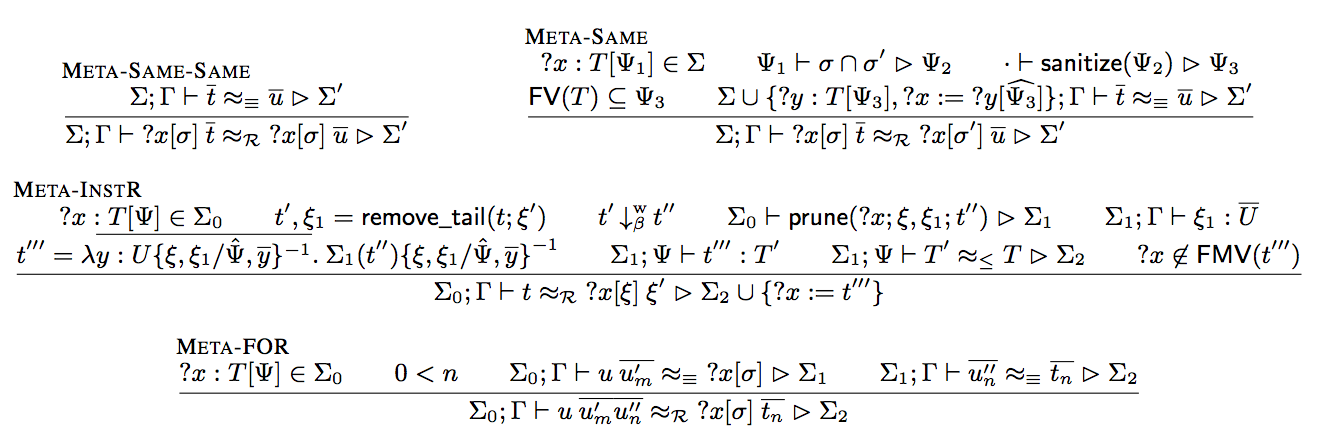
\includegraphics[width=0.8\textwidth]{fig/coq.png}
            ~\footnote{Ziliani, Beta, and Matthieu Sozeau. "A unification
              algorithm for Coq featuring universe polymorphism and
              overloading." ACM SIGPLAN Notices. Vol. 50. No. 9. ACM, 2015.}
        \end{figure}
        }
    \only<2->{
    \item<2-> Developments on dependent type systems that give programmers more control.
      \begin{itemize}
        \item Manage type-level computations using explicit casts.
          \only<2-2>{
            \footnote{Yang, Yanpeng, Xuan Bi, and Bruno C. D. S. Oliveira.
              "Unified Syntax with Iso-types." Asian Symposium on Programming
              Languages and Systems. Springer International Publishing, 2016.}
            \footnote{van Doorn, Floris, Herman Geuvers, and Freek Wiedijk.
              "Explicit convertibility proofs in pure type systems." Proceedings
              of the Eighth ACM SIGPLAN international workshop on Logical
              frameworks \& meta-languages: theory \& practice. ACM, 2013.}
            \footnote{Kimmell, Garrin, et al. "Equational reasoning about
              programs with general recursion and call-by-value semantics."
              Proceedings of the sixth workshop on Programming languages meets
              program verification. ACM, 2012.}
            \footnote{Sjöberg, Vilhelm, and Stephanie Weirich. "Programming up
              to congruence." ACM SIGPLAN Notices. Vol. 50. No. 1. ACM, 2015.}
            }
        \item Decidable type checking based on alpha-equality.
        \item Easy to combine recursive types.
      \end{itemize}
      \only<2-2>{
        \begin{figure}[ht]
          \begin{center}
            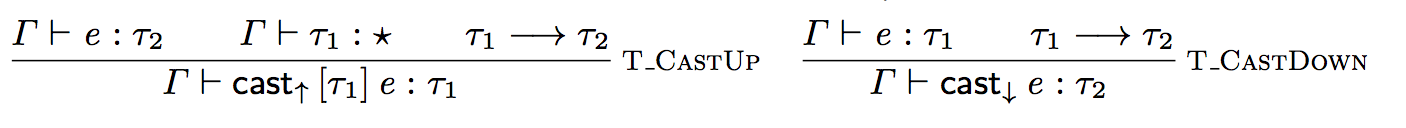
\includegraphics[width=0.8\textwidth]{fig/cast.png}
          \end{center}
        \end{figure}
      }
    \item<3-> Question: can we get rid of the complication of the algorithms in
      those systems?
    }
  \end{itemize}
\end{frame}

%% frame : Goals and non-goals

\newcommand\hl[1]{{\color{blue} #1}}

\begin{frame}
  \frametitle{Goals}
  Our goal is to
  \begin{itemize}
  \item present a \hl{simple and complete} unification algorithm for
    \hl{first-order} dependent type systems with \hl{alpha-equality} based type
    checking
  \item fill the gap between delicate unification algorithms for simple types
    and sophisticated unification algorithms for dependent types.
  \end{itemize}
  We do \textit{not} intend to
  \begin{itemize}
  \item solve more problems than existing unification algorithms.
  \item serve for beta-equality based dependent type systems.
  \end{itemize}
\end{frame}

%% frame : Contribution

\begin{frame}
  \frametitle{Contributions}
  \begin{itemize}
    \item \hl{Strategy}: \textit{type sanitization} that resolves the
      dependency between types.
    \item \hl{Algorithm}: an alpha-equality based unification algorithm for
      first-order dependent types.
    \item \hl{Extension}: subtyping in implicit polymorphism.
    \item \hl{Meta-theory Study}: undergoing.
  \end{itemize}
\end{frame}

%% frame : bg

\begin{frame}[fragile]
  \frametitle{Background: Dependent Types}
  \begin{itemize}
    \item Types depends on terms.
    \item Vector of integers
      \begin{itemize}
        \item definition without dependent types:
          $data ~ Vect = Nil~|~Cons~Int~Vect$
          \begin{itemize}
            \item<2-> one definition that could cause \hl{run-time error}\\
              $head :: Vect \to Int$
            \item<3-> make it \hl{total}\\
              $head :: Vect \to Maybe~Int$
          \end{itemize}
        \item<4-> definition with dependent type: \hl{sized} Vector\\
      \begin{lstlisting}
data Vect :: Nat -> Type  =
  | Nil :: Vect Z
  | Cons :: Int -> Vect k -> Vect (S k)
      \end{lstlisting}
      \begin{overlayarea}{\linewidth}{1cm}
        \begin{onlyenv}<5->
          \begin{lstlisting}
       head :: Vect (S k) -> Int
          \end{lstlisting}
      \end{onlyenv}
      \end{overlayarea}
      \end{itemize}
  \end{itemize}
\end{frame}

%% frame : bg

\begin{frame}
  \frametitle{Background: Unification Problem}
  \begin{block}{Unification}
  Given \hl{two terms} containing some unification variables,
  find the \hl{substitution}
  which makes two terms \hl{equal}.
  \end{block}

  \uncover<2->{
  \begin{itemize}
    \item $\genA \to Int$
    \item $Bool \to Int$
  \end{itemize}
  }

  \uncover<3->{
  Solution: $\genA = Bool$.
  }
\end{frame}

%% frame : Unification Algorithm

\section{Unification Algorithm}
\begin{frame}{Outline}
\tableofcontents[currentsection]
\end{frame}

\begin{frame}{Language}
  \begin{itemize}
    \item \hl{Unified syntax} based on $\lambda C$
  \begin{block}{Syntax}
    \begin{tabular}{lrcl}
  Type & $\sigma, \tau$ & \syndef & $\genA \mid e$ \\
  Expr & $e$ & \syndef & $x \mid \star \mid e_1~e_2 \mid \blam x \sigma e \mid \bpi x {\sigma_1} \sigma_2$ \\
    \end{tabular}
  \end{block}
  \item $\erlam x e \equiv \blam x \genA e$
  \item Example: $(\blam x \star {\blam y {\hl{x}} y}) :: \bpi x \star {\bpi y x x}$
  \item $A \to B$ for $\bpi x A B$ if $x$ does not appear in $B$.
  \end{itemize}
\end{frame}

\begin{frame}{Unification Algorithm}
  Key ideas:
  \begin{itemize}
  \item \hl{ordered} algorithmic typing context
    ~\footnote{Dunfield, Joshua, and Neelakantan R. Krishnaswami. "Complete and
      easy bidirectional typechecking for higher-rank polymorphism." ACM SIGPLAN
      Notices. Vol. 48. No. 9. ACM, 2013.}:
    \begin{block}{Algorithmic typing context}
      Contexts
      $\tctx, \ctxl, \ctxr$  \syndef $\ctxinit \mid \tctx,x:\sigma
      \mid \tctx, \hl{\genA}
      \mid \tctx, \hl{\genA = \tau} $
    \end{block}
    scope constraint
    \begin{itemize}
      \item $\blam x \genA {\blam y \genB} y$
      \item $\genA = y$ \alert{invalid}
      \item $\genB = x$ \hl{valid}
    \end{itemize}
  \item<2-> \hl{judgment}: $\tctx \byuni \tau_1 \uni \tau_2 \hl{\toctx}$
  \item<3-> invariant: inputs are already \hl{fully substituted} under current context.
    \begin{itemize}
      \item $\genA = \Int \byuni \genA \uni \Bool$ \alert{invalid}
      \item $\genA = \Int \byuni \Int \uni \Bool$
    \end{itemize}
  \end{itemize}
\end{frame}

\begin{frame}{Problem}
  The case when we have a unification variable on one side:
  \begin{itemize}
    \item $\hl{\tctx}, \genA, \ctxr \byinf \genA \uni \tau$
    \item<2-> what we will do if $\tau$ is a function?
       $\tctx_1, \genA, \tctx_2 \byuni \genA \uni A \to B$
      \begin{itemize}
        \item<3-> try directly scope constraint? \alert{No.}
        \item<4-> $\genA, \hl{\genB} \byuni \genA \uni \Int \to \hl{\genB}$
        \item<5-> $\hl{\genA_1}, \genA = \Int \to \hl{\genA_1}, \genB = \hl{\genA_1}$
        \item<6-> \hl{unification variables need special treatments in scope constraint}!
      \end{itemize}
    \item<7-> In Dunfield and Krishnaswami 2013
      ~\footnote{Dunfield, Joshua, and Neelakantan R. Krishnaswami. "Complete and
        easy bidirectional typechecking for higher-rank polymorphism." ACM SIGPLAN
        Notices. Vol. 48. No. 9. ACM, 2013.}:
      \begin{itemize}
        \item<8-> solve $\genA = \genA_1 \to \genA_2$.
        \item<8-> unify
          $\tctx_1, \genA_1, \genA_2, \genA = \genA_1 \to \genA_2, \tctx_2 \byuni \hl{\genA_1 \uni A}$\\
          ~~~~~~~$\tctx_1, \genA_1, \genA_2, \genA = \genA_1 \to \genA_2, \tctx_2 \byuni \hl{\genA_2 \uni B}$
      \end{itemize}
    \item<9-> Then $\tctx_1, \genA, \tctx_2 \byuni \genA \uni \bpi x \star \hl{x}$?
      \begin{itemize}
        \item<10-> $\genA_2 = x$
        \item<11-> $\tctx_1, \genA_1, \alert{x}, \genA_2, \genA = \genA_1 \to
          \genA_2, \alert<12->{\tctx_2}.$ \uncover<13->{\alert{No.}}
      \end{itemize}
  \end{itemize}
\end{frame}

\begin{frame}{Problem}
  \begin{itemize}
    \item can not use scope constraint directly because of unification variables
      \begin{itemize}
        \item $\genA, \hl{\genB} \byuni \genA \uni \Int \to \hl{\genB}$
        \item $\hl{\genA_1}, \genA = \Int \to \hl{\genA_1}, \genB = \hl{\genA_1}$
      \end{itemize}
    \item cannot destruct a Pi type because of the type dependency
      \begin{itemize}
      \item $\tctx_1, \genA, \tctx_2 \byuni \genA \uni \bpi x \star \hl{x}$
      \end{itemize}
    \item<2-> observation: we can always solve it by \hl{a fresh unification
      variable} that satisfies the scope constraint.
    \item<3-> Our solution:
        for unification problem
        $\tctx, \genA, \ctxr \byinf \genA \uni \tau$,
        we \hl{sanitize} the unification variables in $\tau$ before we check the
        scope constraint.
  \end{itemize}
\end{frame}

\begin{frame}{Strategy}
  \begin{block}{Type Sanitization}
    Given $\genA, \tau$, solve unification variables in $\tau$ out of scope of
    $\genA$ by fresh unification variables that in that scope of $\genA$.
  \end{block}
  \uncover<2->{Example}
  \begin{itemize}
  \item<3-> $\genA, \genB \byuni \genA \uni \Int \to \genB$
    \begin{itemize}
      \item type sanitization: $\genA, \genB \bycg \Int \to \genB \cgto \Int \to
        \genA_1 \dashv \hl{\genA_1}, \genA, \hl{\genB = \genA_1}$
      \item solution: $\genA_1, \genA = \Int \to \genA_1, \genB = \genA_1$
    \end{itemize}
  \item<4-> $\genA, \genB, x \byuni \genA \uni x \to \genB$
    \begin{itemize}
      \item<5-> type sanitization: $\genA, \genB \bycg \alert<6->{x} \to \genB
        \cgto \alert<6->{x} \to
        \genA_1 \dashv \hl{\genA_1}, \genA, \hl{\genB = \genA_1}$
      \item<6-> solution: \alert{fail}.
    \end{itemize}
  \end{itemize}
\end{frame}

\begin{frame}{Unification}
  Key ideas:
  \begin{itemize}
    \item \hl{ordered} algorithmic typing context. \hl{scope constraint}.
    \item \hl{judgment}: $\tctx \byuni \tau_1 \uni \tau_2 \toctx$
    \item invariant: inputs are already \hl{fully substituted} under current
      context.
    \item<2-> strategy: \hl{type sanitization}
  \end{itemize}
  \uncover<3->{...Find more explanations in the paper.}
\end{frame}

\section{Extension: Implicit polymorphism}

\begin{frame}{Outline}
  \tableofcontents[currentsection]
\end{frame}


\begin{frame}{Language}
    \begin{block}{Syntax}
      \begin{tabular}{lrcl}
        Type & $\sigma $ & \syndef & $\genA \mid e$ \\
        Expr & $e$ & \syndef & $x \mid \star \mid e_1~e_2 \mid \blam x \sigma e \mid \bpi x {\sigma_1} \sigma_2$ \\
             && \synor & $\hl{\forall x: \star. \sigma}$ \\
        \hl{Monotype} & $\tau$ & \syndef & $ \{ \sigma' \in \sigma, \forall \notin \sigma'\} $ \\
      \end{tabular}
    \end{block}
    \begin{itemize}
    \item A \hl{restricted} version of polymorphic types.
    \item We write $\forall a. a \to a$ for $\forall a: \star. a \to a$.
    \item<2-> \hl{Predictivity}: universal quantifiers can only be instantiated by monotypes.
    \item<3-> Unification is between monotypes.
    \item<3-> Unification variables can only have monotypes.
    \end{itemize}
\end{frame}

\begin{frame}{Subtyping}
  \begin{block}{Polymorphic Subtyping}
    $\sigma_1$ is a subtype of $\sigma_2$, denoted by $\tctx \bysub \sigma_1 \lt
    \sigma_2$,
    if $\sigma_1$ is more polymorphic than $\sigma_2$ under $\tctx$.
  \end{block}

  \begin{itemize}
  \item examples:
    \begin{itemize}
      \item $\tctx \bysub \forall a. a \to a \tsub \Int \to \Int$
      \item $\tctx \bysub \Int \to (\forall a. a \to a) \tsub \Int \to (\Int \to
        \Int)$
      \item $\tctx \bysub (\Int \to \Int) \to \Int \tsub (\forall a. a \to a) \to \Int$
    \end{itemize}
  \end{itemize}
\end{frame}

\begin{frame}{Problem}
  What happen if we have a unification variable on one side?
  \begin{itemize}
  \item<2-> do unification?
\begin{mathpar}
\inferrule{\tpreuni \genA \uni \sigma \toctx}{\tpresub \genA \lt \sigma \toctx}
\end{mathpar}
  \item<3-> unification variables can only be solved by \hl{monotypes}!
  \item<4-> however, we cannot restrict $\sigma$ to be a monotype
    \begin{mathpar}
\tpresub \genA \lt \bpi x {(\forall y .y \to y)} \Int
    \end{mathpar}
    with solution $\genA = \bpi x {(\Int \to Int)} \Int$
  \item <5-> again, we \hl{cannot} destruct pi type because of type
    dependency.
    \begin{mathpar}
\tpresub \genA \lt \bpi x \star x
    \end{mathpar}
  \end{itemize}
\end{frame}

\begin{frame}{Problem}
  \begin{itemize}
    \item $\tpresub \genA \lt \bpi x {\alert<2->{(\forall y .y \to y)}} \Int$\\
      with solution $\genA = \bpi x {\alert<2->{(\Int \to Int)}} \Int$
    \item<2-> Observation:
      when the unification variable is \hl{on the left},
      even though there can be polymorphic components \hl{on the right},
      those polymorphic components must appear \hl{contra-variantly}.
    \item<3-> similar observation for when the unification variable on the right,
      polymorphic components must appear \hl{co-variantly}.
    \item<4-> $\genA = \bpi x {\alert{(\Bool \to \Bool)}} \Int$
    \item<5-> $\genA = \bpi x {\alert{(\genA_1 \to \genA_1)}} \Int$
    \item<6-> How to turn $\bpi x {\hl{(\forall y .y \to y)}} \Int$
      into $\bpi x {\hl{(\genA_1 \to \genA_1)}} \Int$
  \end{itemize}
\end{frame}

\begin{frame}{Strategy}
  \begin{itemize}
  \item How to turn $\bpi x {(\forall \hl{y} .\hl{y} \to \hl{y})} \Int$
    into $\bpi x {(\hl{\genA_1} \to \hl{\genA_1})} \Int$
  \item we can always replace universal quantifiers that appear contra-variantly
    by a fresh unification variable.
  \item<2-> our solution: for subtyping problem between $\genA$ and $\sigma$, we
      \hl{sanitize} the contra-variant universal quantifiers in $\sigma$ before we
      use unification.
  \end{itemize}
\end{frame}

\begin{frame}{Strategy}
  \begin{block}{Polymorphic Type Sanitization}
    Given $\genA, \sigma$, remove universal quantifiers appearing
    contra-variantly, and replace corresponding type variables by a fresh
    unification variable.
  \end{block}
  \uncover<2->{Example}
  \begin{itemize}
  \item<2-> $\genA \bysub \genA \tsub (\forall a. a \to a) \to \Int$
    \begin{itemize}
      \item<3-> polymorphic type sanitization: $\genA \bycg (\forall a. a \to a) \to
        \Int \cgto (\hl{\genA_1} \to \hl{\genA_1}) \to \Int \dashv \hl{\genA_1}, \genA$
      \item<4-> after unification: $\genA_1, \genA = (\hl{\genA_1} \to \hl{\genA_1})
        \to \Int$
    \end{itemize}
  \item<5-> $\genA \bysub \genA \tsub (\forall a. a \to a)$
    \begin{itemize}
      \item<6-> polymorphic type sanitization \alert{fail.}
    \end{itemize}
  \item<7-> $\genA, \genB \bysub \genA \tsub \Int \to \genB$
    \begin{itemize}
      \item<8-> polymorphic type sanitization: $\genA, \genB \bycg \Int \to \genB
        \cgto \Int \to \genB \dashv \genA, \genB$
      \item<9-> unification: $\hl{\genA_1}, \genA = \Int \to \genA_1, \genB = \genA_1$
    \end{itemize}
  \item<10-> Find more explanations in the paper!
  \end{itemize}
\end{frame}

\section{Conclusion}

\begin{frame}{Outline}
\tableofcontents[currentsection]
\end{frame}

\begin{frame}{Related Work}
  \begin{itemize}
\item \hl{Powerful but complicated} unification algorithms for dependent types:
  \begin{itemize}
  \item Ziliani, B., Sozeau, M. (2015, August)
  \footnote{Ziliani, Beta, and Matthieu Sozeau. "A unification algorithm for Coq
    featuring universe polymorphism and overloading." ACM SIGPLAN Notices. Vol.
    50. No. 9. ACM, 2015.};
  Elliott, C. (1989).
  \footnote{Elliott, Conal. "Higher-order unification with dependent function
    types." Rewriting Techniques and Applications. Springer Berlin/Heidelberg,
    1989.};
  Abel, A., Pientka, B. (2011, June)
  \footnote{Abel, Andreas, and Brigitte Pientka. "Higher-order dynamic pattern
    unification for dependent types and records." International Conference on
    Typed Lambda Calculi and Applications. Springer Berlin Heidelberg, 2011.}
  \end{itemize}
\item Complete and easy unification/subtyping algorithm for \hl{simple types and
  System F types}:
  \begin{itemize}
  \item Hindley-Milner algorithm
    \footnote{Damas, Luis, and Robin Milner. "Principal type-schemes for
      functional programs." Proceedings of the 9th ACM SIGPLAN-SIGACT symposium
      on Principles of programming languages. ACM, 1982.}
    \footnote{Hindley, Roger. "The principal type-scheme of an object in
      combinatory logic." Transactions of the american mathematical society 146
      (1969): 29-60.};
  Dunfield, J., Krishnaswami, N. R. (2013, September).
    \footnote{Dunfield, Joshua, and Neelakantan R. Krishnaswami. "Complete and
      easy bidirectional typechecking for higher-rank polymorphism." ACM SIGPLAN
      Notices. Vol. 48. No. 9. ACM, 2013.};
  Jones, S. P., Vytiniotis, D., Weirich, S., Shields, M. (2007)
    \footnote{Jones, Simon Peyton, et al. "Practical type inference for
      arbitrary-rank types." Journal of functional programming 17.01 (2007):
      1-82.};
  \end{itemize}
\item Dependent type systems with \hl{alpha-equality} based type checking:
  \begin{itemize}
  \item type-level computation by explicit casts
            \footnote{Yang, Yanpeng, Xuan Bi, and Bruno C. D. S. Oliveira.
              "Unified Syntax with Iso-types." Asian Symposium on Programming
              Languages and Systems. Springer International Publishing, 2016.}
            \footnote{van Doorn, Floris, Herman Geuvers, and Freek Wiedijk.
              "Explicit convertibility proofs in pure type systems." Proceedings
              of the Eighth ACM SIGPLAN international workshop on Logical
              frameworks \& meta-languages: theory \& practice. ACM, 2013.}
            \footnote{Kimmell, Garrin, et al. "Equational reasoning about
              programs with general recursion and call-by-value semantics."
              Proceedings of the sixth workshop on Programming languages meets
              program verification. ACM, 2012.}
            \footnote{Sjöberg, Vilhelm, and Stephanie Weirich. "Programming up
              to congruence." ACM SIGPLAN Notices. Vol. 50. No. 1. ACM, 2015.}
  \end{itemize}
\end{itemize}
\end{frame}

\begin{frame}{Conclusion}
\begin{itemize}
  \item \hl{Strategy}: a both simple to understand and simple
    to implement strategy called \textit{type sanitization}
  \item \hl{Algorithm}: A simple and complete alpha-equality based unification
    algorithm
  \item \hl{Extension}: \textit{polymorphic type sanitization} to deal with
    polymorphic subtyping.
  \item \hl{Meta-theory}: proof sketches.
\end{itemize}
\end{frame}

\begin{frame}
  \begin{center}
  \Huge Thanks for listening!
  \end{center}
\end{frame}

\end{document}